\documentclass[dvipsnames]{beamer}


\usepackage[utf8]{inputenc}
\usepackage[T1]{fontenc}

\usepackage{lmodern} % get rid of fontsize warning
\usepackage{tikz}
%\usetikzlibrary{calc,chains,shapes,positioning}
\usepackage{pgfplots}
\pgfplotsset{compat=1.18}
\usepackage{verbatim}
\usepackage{amsmath}
\usepackage{textpos}
\usepackage{gradient-text}
% \usepackage[dvipsnames]{xcolor}
\usepackage{graphicx}
\usepackage[normalem]{ulem}
%\usepackage[colorlinks=false,pdfborder={0 0 0}]{hyperref}



\title{git - the stupid content tracker}
\subtitle{git eats trees.}
\author{Henry S. {Grasshorn Gebhardt}}
%\institute[The Pennsylvania State University]
%{Department of Astronomy and Astrophysics}
%\date{February 26, 2013}



\newcommand{\comp}[1]{{\tt #1}}


\begin{document}

\frame{\titlepage}

\section[Outline]{}
\frame{
    \frametitle{Outline}
    \tableofcontents
}


\section{Introduction to Version Control}
\frame{
    \frametitle{Version Control? Version Control.}
    % Premise: Code is text.

    % \bigskip
    Version control helps to:
    \begin{itemize}
        \item Save history.
        \item Keep track of changes.
        \item Merge code.
        \item Share code. (Don't be a git!)
        \item Consistency checking, e.g., when running code or configs elsewhere.
        \item \ldots
    \end{itemize}

    Git, Mercurial, \sout{Bazaar}, \sout{SVN (why bother?)}, \sout{CVS},
    \sout{Monotone}, \sout{DARCS}, \ldots

    ``Theory of Patches''
}

\frame{
    \frametitle{Git was created by Linus Torvalds for Linux kernel development}

    Linux developers used to use \texttt{BitKeeper} until it wasn't free anymore.

    \smallskip

    So Linus Torvalds created git, which always had a reputation for being too
    complicated to use. First release 7 April 2005.

    \smallskip

    There are {\color{red}\emph{plumbing}} commands and
    {\color{blue}\emph{porcelain}} commands.

    \smallskip

    \centering
    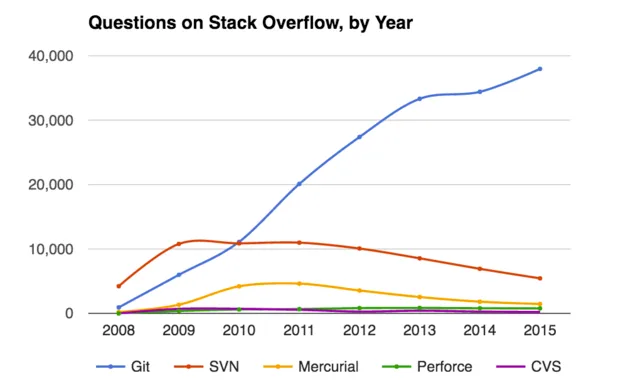
\includegraphics[width=0.7\textwidth]{./git-so}
}


\frame{
    \frametitle{What is a patch?}

    Patches are text files that show \gradientRGB{cha}{10,10,255}{100,255,10}\gradientRGB{nges}{100,255,10}{255,10,10}.

    \bigskip

    {\color{Green} Create a patch:}\\
    \texttt{\$ diff -Naur file1 file2 > changes.patch}
    \medskip

    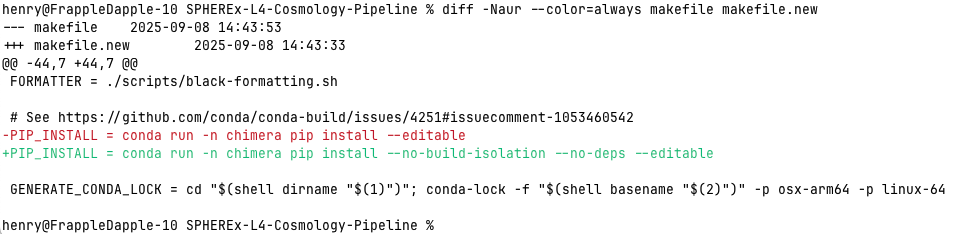
\includegraphics[width=\textwidth]{create_patch.png}

    \bigskip

    {\color{blue} Apply a patch:}\\
    \texttt{\$ patch -p1 < changes.patch}
}


\section{Theory}
\frame{
    \frametitle{Git History}

    \begin{center}
        \url{https://git-scm.com}
    \end{center}
    \bigskip

    History is a DAG (directed acyclic graph). \emph{Explain graph.}
    \bigskip

    Distributed, not centralized. \emph{Every clone has the full history.}
    \bigskip

    % There are \emph{plumbing} commands and \emph{porcelain} commands.
}

\frame{
    \frametitle{Git doesn't know about directories\ldots whaaat?}

    Git only knows content. (blobs)
    \bigskip

    How that content is assembled. (trees)
    \bigskip

    And history. (commits)
    \bigskip

    Each commit stores the full source code (no patches!).
}


\frame{
    \frametitle{blobs, trees, and commits are identified by their SHA1-sum}

    \hfill 9fc058eae64b097d7a270a404527375526e65cea \hfill
    \bigskip
    \bigskip

    A hash is a (hopefully) unique number to identify some information, like a
    file.
    \medskip

    SHA-1 is a 160-bit number. It happens to be cryptographically secure.
    \medskip

    Blobs, trees, and commits are identified by their SHA1 sum.
    \medskip

    $\Rightarrow$ Efficient de-duplication and compression
}


\frame{
    \frametitle{Terminology: blah, blah, blah,\ldots}
    WORKDIR (directory where files are checked out) \\
    GITDIR (\texttt{.git}) \\
    HEAD (currently checked out commit) \\
    Index (staging area for next commit) \\
    Local repository \\
    Upstream repository \\
    Stash
}


\section{git commands}

\frame{
    \frametitle{Per-seat Initialization}
    Initialization once per machine ({\tt \char`~/.gitconfig}):
    \begin{quote}
        \tt
        \$ git config -$\,$-global user.name "Henry VIII" \\
        \$ git config -$\,$-global user.email "h@here.com"
    \end{quote}

    \bigskip

    Set your {\tt EDITOR} variable in {\tt \char`~/.bashrc} or {\tt
    \char`~/.profile} or wherever you set your environment variables.
}


\frame{
    \frametitle{Making history}
    First, add changes to staging area (the \emph{index}):
    \begin{description}[Other]
        \item[git add <file>]  \# Add your changes to the index.
        \item[git add -p] \hspace{0.6cm} \# Be selective about what to add.
    \end{description}

    \bigskip
    Then, commit:
    \begin{description}[Other]
        \item[git commit]  \# Commits your changes.
    \end{description}
    Add a short title, and then a longer description.
}


\section{Workflows and git branches}
\frame{
    \frametitle{What to commit}
    \begin{itemize}
        \item The bare minimum to recreate the project.
        \item Plots! (They are the minimum to recompile the \LaTeX{}.)
    \end{itemize}

    \bigskip
    \bigskip
    \texttt{.gitignore} can appear anywhere in the git repository, and contains
    files to ignore, e.g.,
    \begin{description}[Other]
        \item[.gitignore]\phantom{0}\\
            *.aux \\
            *.log \\
            *.toc \\
    \end{description}

    \bigskip
    Reasons: avoid conflicts, save space.
}


\frame{
    \frametitle{Where to commit: Branches}
    \begin{description}
        \item[\emph{master} (or \emph{main}):] Main development branch.
        \item[release branches:] More stable branches that you might want to
            keep supporting by fixing bugs and cherry-picking commits from
            \emph{master}.
        \item[feature branches:]  Development branch for specific features. By
            convention, they often start with your initials, e.g.,
            \emph{hg/integration\_method\_B}. Should eventually be merged into
            \emph{master}.
    \end{description}
}

\frame{
    \frametitle{Trees, yum!}
    \framesubtitle{git eats trees\ldots nom,nom}

    Branches are cheap!

    \bigskip
    \begin{description}
        \item[git branch -a] List branches.
        %\item[git branch -d <name>] Delete a branch.
        %\item[git checkout <name>] Let's climb over to that branch.
        \item[git checkout {[}-b <newbranch>{]} <starthere>] Checkout and make a new branch.
        \item[git merge <otherbranches>...] Trees eating trees!
        \item[git rebase -i <branchname>] Clean up your history!
    \end{description}
}


\frame{
    \frametitle{Pushing and pulling}
    \color{red} Put graph of distributed computing.

    {\tt
        \hspace{1cm}\$ git push <remote> <localbranch>:<remotebranch> \\
        \hspace{1cm}\$ git push -$\,$-set-upstream \\
        \hspace{1cm}\$ git pull \\
        \hspace{1cm}\$ git remote -v \\
    }
}


\section{Clones and Remote Repositories}
\frame{
    \frametitle{Each git clone is a full repository}

    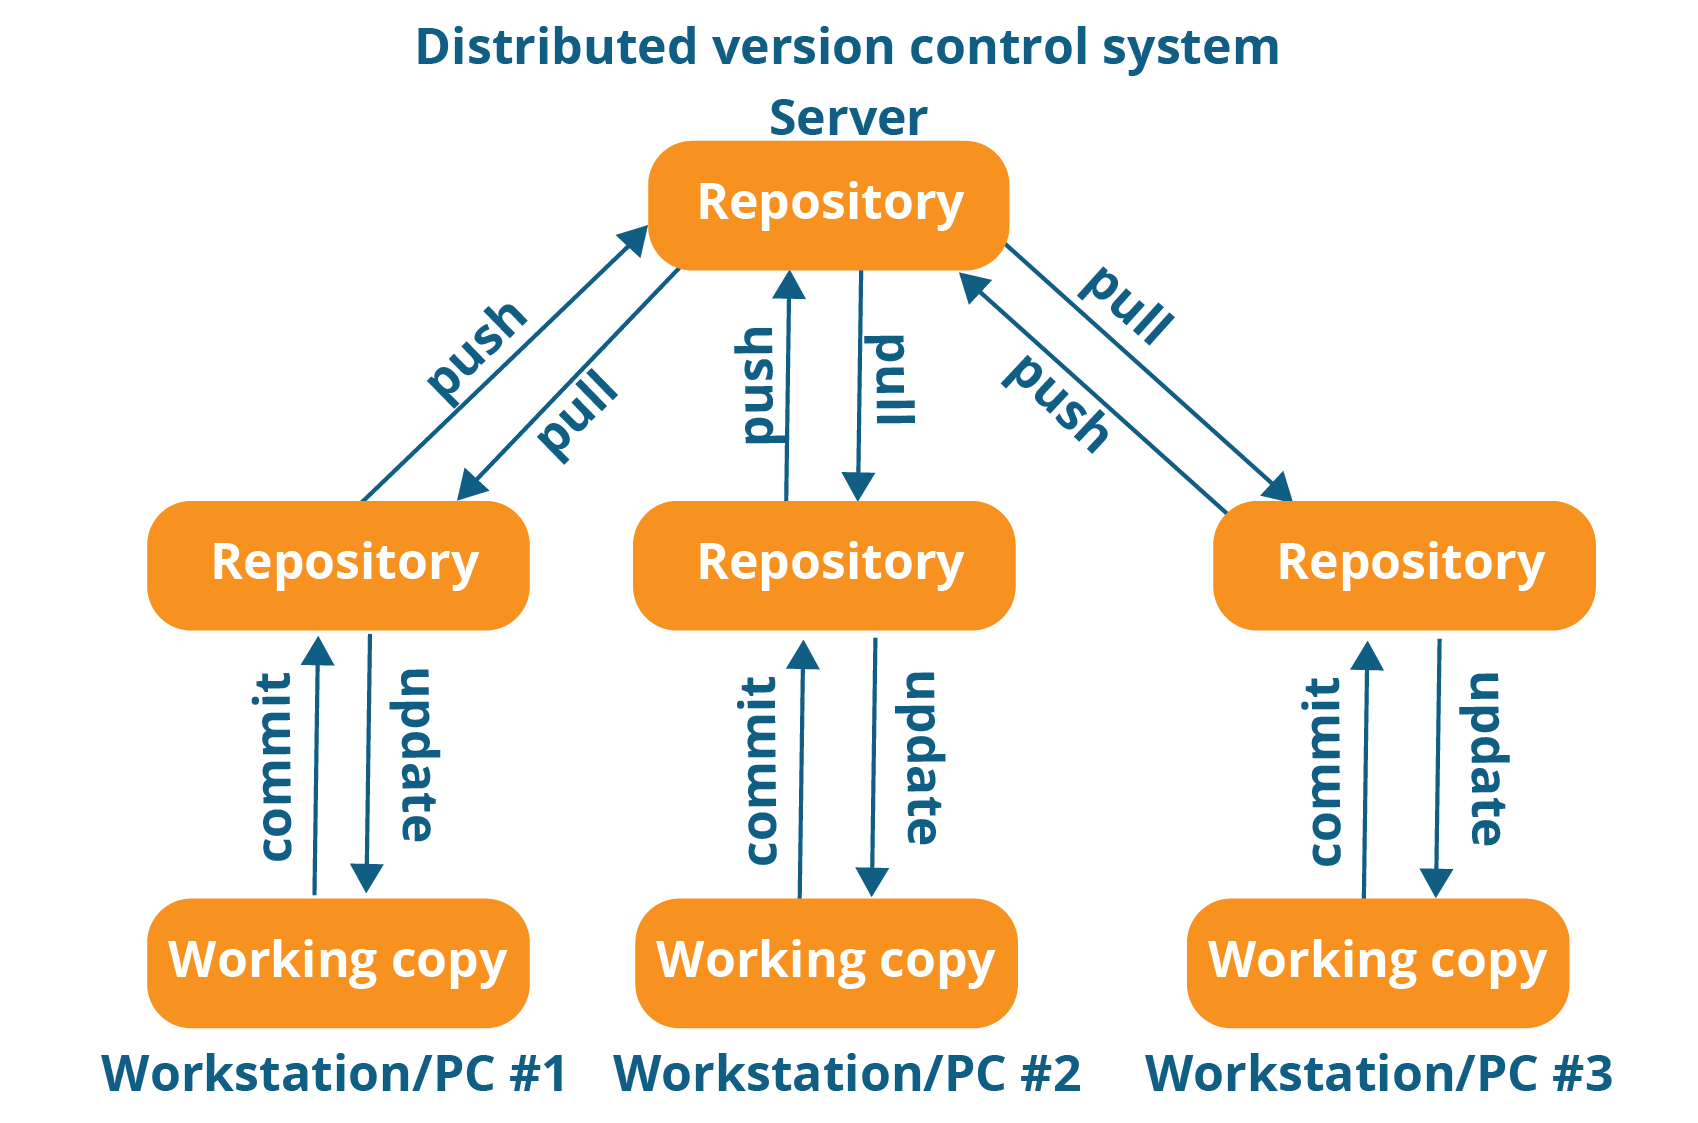
\includegraphics[width=\textwidth]{Distributed-Version-Control-System-Workflow-What-Is-Git-Edureka.png}

    \texttt{git pull} = \texttt{git fetch} + \texttt{git merge}
}


\frame{
    \frametitle{Pull Requests (PR) and merging}
    PRs are used to coordinate work between multiple people.

    \bigskip
    \bigskip
    \bigskip

    Best kind of merge is a fast-forward: no merging, no conflicts!
    \begin{description}
        \item[git merge <branchnames>...] Merge branches.
        \item[git mergetool] Resolve conflicts.
    \end{description}
}


\frame{
    \frametitle{Play nice together!}
    \begin{center}
        {\tt \$ git svn}
        \vfill
        Works by calling ``{\tt git fast-import}''.
    \end{center}
}

\frame{
    \frametitle{Upstreams and tracking branches}
    A branch can be set to track an upstream:
    \bigskip

    \mbox{\hspace{-0.5cm}\texttt{git push -$\,$-set-upstream origin <localbranch>:<remotebranch>}}
}



\section{Summary and cheatsheet}

\frame{
    \frametitle{git cheat sheet}

    Here's the \emph{porcelain}:
    \bigskip

    %\url{https://services.github.com/kit/downloads/github-git-cheat-sheet.pdf}
    \url{https://about.gitlab.com/images/press/git-cheat-sheet.pdf}

    \vfill

    {\tt man gittutorial}

    \vfill
    Initialization once per machine:\\
    \hspace{1cm}Create the file {\tt \char`~/.gitconfig}.

    Set your {\tt EDITOR} variable in {\tt \char`~/.bashrc} or {\tt \char`~/.profile}.
}


\appendix
\frame{
    \centering \huge \color{blue}{Appendix}
}

\frame{
    \frametitle{git cheat sheet}

    Here's the \emph{porcelain}:
    \bigskip

    %\url{https://services.github.com/kit/downloads/github-git-cheat-sheet.pdf}
    \url{https://about.gitlab.com/images/press/git-cheat-sheet.pdf}
}


\frame{
    \frametitle{Directory structure}
    \frametitle{git stores its information in a .git directory}
    {\tt
        \hspace{1cm}newrepo/ \\
        \hspace{1.5cm}    .git/ \\
        \hspace{1.5cm}    .gitignore \\
        \hspace{1.5cm}    README.md \\
        \hspace{1.5cm}    doc/ \\
        \hspace{1.5cm}    src/ \\
        \hspace{1.5cm}    test/ \\
    }
}


\frame{
    \frametitle{git help command}

    Useful commands:

    \begin{description}[Other]
        \item[git status] Where am I?
        \item[git diff] What did I just do?
        \item[git diff -$\,$-staged] What will I do?
        \item[git log] What have I done?
        \item[gitk -$\,$-all] Let's climb trees!
        \item[git describe -$\,$-always -$\,$-tags -$\,$-dirty] Who am I?
    \end{description}
}

\frame{
    \frametitle{Pushing and pulling}
    {\tt
        \hspace{1cm}\$ git push <remote> <localbranch>:<remotebranch> \\
        \hspace{1cm}\$ git push -$\,$-set-upstream \\
        \hspace{1cm}\$ git pull \\
        \hspace{1cm}\$ git remote -v \\
    }
}

\frame{
    \frametitle{Initial checkout}
    Existing repository:
    {\tt\\
        \hspace{0.3cm}\$ git clone <url>
    }
    \vfill
    New repository:
    {\tt\\
        \hspace{1cm}\$ mkdir newrepo\\
        \hspace{1cm}\$ cd newrepo\\
        \hspace{1cm}\$ git init
    }
}

\frame{
    \frametitle{Sending and receiving patches}
    \begin{description}[Other]
        \item[git format-patch] Create a patch
        \item[git send-email] Send an entire set of patches as emails.
        \item[git am, git apply] Apply other people's patches.
    \end{description}
}

\frame{
    \frametitle{Merging branches and conflicts}
    {\tt git mergetool}
}


\frame{
    \frametitle{Ah, I did something stupid\ldots}

    Recovery might be possible by looking into {\tt .git/logs/}.

    \bigskip
    {\tt git reflog} parses it for you.
}


\frame{
    \frametitle{Other commands}

    Graphs: {\tt git log -$\,$-graph}
    \bigskip

    More graphs: {\tt gitk -$\,$-all}
    \bigskip

    Tags: {\tt git tag}
    \bigskip

    Hooks: {\tt man githooks}; {\tt cd .git/hooks/}
    \bigskip

    Submodules: {\tt git submodule}
    \bigskip

    Rewrite history: {\tt  git filter-branch}
    \bigskip

    Collect garbage: {\tt git gc}
}


\section{Hosting (github, gitlab, forgejo, gitolite, \ldots)}

\frame{
    \frametitle{Hosting your git repository}
    Companies:
    \begin{itemize}
        \itemindent3em
        \item[Github:] \url{github.com}
        \item[Gitlab:] \url{gitlab.com}
        \item[Sourcehut:] \url{sourcehut.org}
        \item[\ldots]
    \end{itemize}
    \bigskip
    Your own:
    \begin{itemize}
        \itemindent3em
        \item[SSH server:] Your own workstation/server.\\
            {\tt
                \hspace{1cm}\$ mkdir -p \char`~/repos/newawesomeproject.git\\
                \hspace{1cm}\$ cd \char`~/repos/newawesomeproject.git\\
                \hspace{1cm}\$ git init -$\,$-bare
            }
        \item[SSH server:] \url{http://gitolite.com/} (Fine-grained permissions)
        \item[Forgejo:] \url{https://forgejo.org/} (Full-on website)
    \end{itemize}
}



\end{document}


% vim: set sw=4 sts=4 et:
